\documentclass[
	a4paper,
	oneside,
	DIV = 12,
	12pt,
	headings = normal,
]{scrartcl}

%%% Length calculations
\usepackage{calc}
%%%

%%% Support for color
\usepackage{xcolor}
\definecolor{lightblue}{HTML}{03A9F4}
\definecolor{red}{HTML}{F44336}
%%%

%%% Including graphics
\usepackage{graphicx}
%%%

%%% Font selection
\usepackage{fontspec}

\setromanfont{STIX Two Text}[
	SmallCapsFeatures = {LetterSpace = 5},
]

\setsansfont{Source Sans Pro}[
]

\setmonofont{Source Code Pro}[
]
%%%

%%% Math typesetting
\usepackage{amsmath}
\usepackage{mathtools}
\usepackage{unicode-math}
\setmathfont{STIX Two Math}

\usepackage[retainorgcmds]{IEEEtrantools}

\DeclarePairedDelimiter{\ceil}{\lceil}{\rceil}

\newcommand*\lnand{\mathbin{\barwedge}}
%%%

%%% Font settings for different KOMAScript elements
\setkomafont{pagenumber}{\rmfamily}
\setkomafont{disposition}{\rmfamily\bfseries}
%%%

%%% Typographic enhancements
\usepackage{microtype}
%%%

%%% Language-specific settings
\usepackage{polyglossia}
\setmainlanguage{ukrainian}
%%%

%%% Captions
\usepackage{caption}
\usepackage{subcaption}

\DeclareCaptionLabelFormat{closing}{#2)}
\captionsetup[subtable]{labelformat = closing}
\captionsetup[subfigure]{labelformat = closing}
%%%

%%% Table typesetting
\usepackage{booktabs}
\usepackage{longtable}

\usepackage{multirow}

\usepackage{array}
\newcolumntype{v}[1]{>{\raggedright\arraybackslash\hspace{0pt}}p{#1}}
\newcolumntype{b}[1]{>{\centering\arraybackslash\hspace{0pt}}p{#1}}
\newcolumntype{n}[1]{>{\raggedleft\arraybackslash\hspace{0pt}}p{#1}}
%%%

%%% SI units typesetting
\usepackage{siunitx}
\sisetup{output-decimal-marker = {,},
exponent-product = {\cdot}}
%%%

%%% TIKZ
\usepackage{tikz}
\usetikzlibrary{arrows.meta, automata, calc, positioning, shapes}
\usetikzlibrary{paths.ortho}

\usepackage{tikzscale}
%%%

%%% Algorithms typesetting
\usepackage[
	ruled,
	linesnumbered,
	onelanguage,
]{algorithm2e}

% Change comments font to roman
\newcommand{\mycommfont}[1]{\rmfamily{#1}}
\SetCommentSty{mycommfont}

% Translate keywords into Ukrainian
\makeatletter
\renewcommand{\listalgorithmcfname}{Список алгоритмів}%
\renewcommand{\algorithmcfname}{Алгоритм}%
\renewcommand{\algocf@languagechoosen}{ukrainian}%

\SetKwBlock{Begin}{початок}{кінець}%
\SetKwIF{If}{ElseIf}{Else}{якщо}{то}{інакше якщо}{інакше}{кінець якщо}%
\makeatother
%%%

%%% Links and hyperreferences
\usepackage{hyperref}
\hypersetup{
	colorlinks      = false,
	linkbordercolor = red,
	urlbordercolor  = lightblue,
	pdfborderstyle  = {/S/U/W 1.5},
}
%%%

%%% Custom commands
\newcommand\schel[1]{\textit{#1}}

\newcommand{\barneg}[1]{\overline{#1}}
%%%

\setlength{\emergencystretch}{1em}

\begin{document}
	\begin{titlepage}
		\begin{center}
			Міністерство освіти і науки України\\
			Національний авіаційний університет\\
			Навчально-науковий інститут комп'ютерних інформаційних технологій\\
			Кафедра комп'ютеризованих систем управління

			\vspace{\fill}
				Розрахунково-графічна робота\\
				з дисципліни «Комп'ютерна схемотехніка»\\

			\vspace{\fill}

			\begin{flushright}
				Виконав:\\
				студент ННІКІТ\\
				групи СП-225\\
				Клокун В.\,Д.\\
				Перевірив:\\
				Іскренко Ю.\,Ю.
			\end{flushright}

			Київ 2018
		\end{center}
	\end{titlepage}

	\section{Завдання}
		Завданням розрахунково-графічної роботи є розробка алгоритму виконання вказаної в завданні операції та синтезу функціональної схеми керуючого автомата.

		\begin{table}[!htbp]
			\centering
			\caption{Завдання на розрахунково-графічну роботу}
			\label{tab:rgr-task}
			\begin{tabular}{lr}
				\toprule
					Параметр & Значення \\
				\midrule
					№                        & 16\\
					Тип операції             & Додавання\\
					Початковий код операндів & ДК\\
					Розрядність операндів    & 16\\
					КВМСМ                    & МДК\\
					Структура ОБ             & ЗМО\\
					Тип автомата             & Мілі\\
					Пам'ять автомата         & $D$\\
					ОР                       & $P$\\
					ЛО                       & \textit{NAND}\\
				\bottomrule
			\end{tabular}
		\end{table}
		З завдання на розрахунково-графічну роботу (табл.~\ref{tab:rgr-task}) видні такі характеристики цільового арифметико-логічного пристрою:
		\begin{enumerate}
			\item Тип арифметичної операції — додавання двійкових чисел.
			\item Початковий код подання операндів~— доповняльний.
			\item Розрядність операндів — 16~біт.
			\item Код виконання операції у суматорі~— доповняльний модифікований.
			\item Структура операційного блока~— із закріпленими мікроопераціями.
			\item Тип керуючого блока~— автомат Мілі з пам'яттю на $D$-тригерах.
			\item Схема логічної ознаки парності молодшого байту.
		\end{enumerate}

	\section{Хід роботи}
		\subsection{Розробка алгоритму}
			Алгоритм додавання двійкових чисел можна словесно описати так:
			\begin{enumerate}
				\item У першому і другому машинних тактах із вхідної шини паралельним кодом записуються операнди~$A$ і~$B$ у відповідні регістри \schel{RGA} і \schel{RGB}. Зчитування операндів здійснюється ЦПК.
				\item Протягом одного машинного такту виконується мікрооперація додавання.
				\item Якщо розрядна сітка не переповнилась, результат записується у регістр~\schel{RGC}.
				\item Якщо розрядна сітка переповнилась, результат не фіксується, і в ЦПК подається сигнал переповнення «ПП».
			\end{enumerate}

		\subsection{Розробка функціональної схеми для виконання додавання}
			Розроблюємо функціональну схему для виконання додавання двох двійкових чисел~(рис.~\ref{fig:01-operational-part-functional-schematic}), яка містить:
			\begin{enumerate}
				\item Регістри \schel{RGA}, \schel{RGB} для приймання і подальшого зберігання першого і другого операндів із вхідної шини \schel{Ш1}.
				\item Паралельний комбінаційний суматор з додатковим старшим розрядом знака~\schel{П} для створення модифікованого доповняльного коду.
				\item Регістр результату~\schel{RGC}, дані з якого пересилаються в оперативну пам'ять по вихідній шині~\schel{Ш2}.
				\item Схеми електронних ключів~\schel{SW1} і~\schel{SW2}.
				\item Схему вироблення ознак переповнення~\schel{OP}.
				\item Схему диз'юнкторів~\schel{OR} для виконання операцій порозрядного логічного додавання кодів операндів~$A$ і~$B$.
			\end{enumerate}

			\begin{figure}[!htbp]
				\centering
				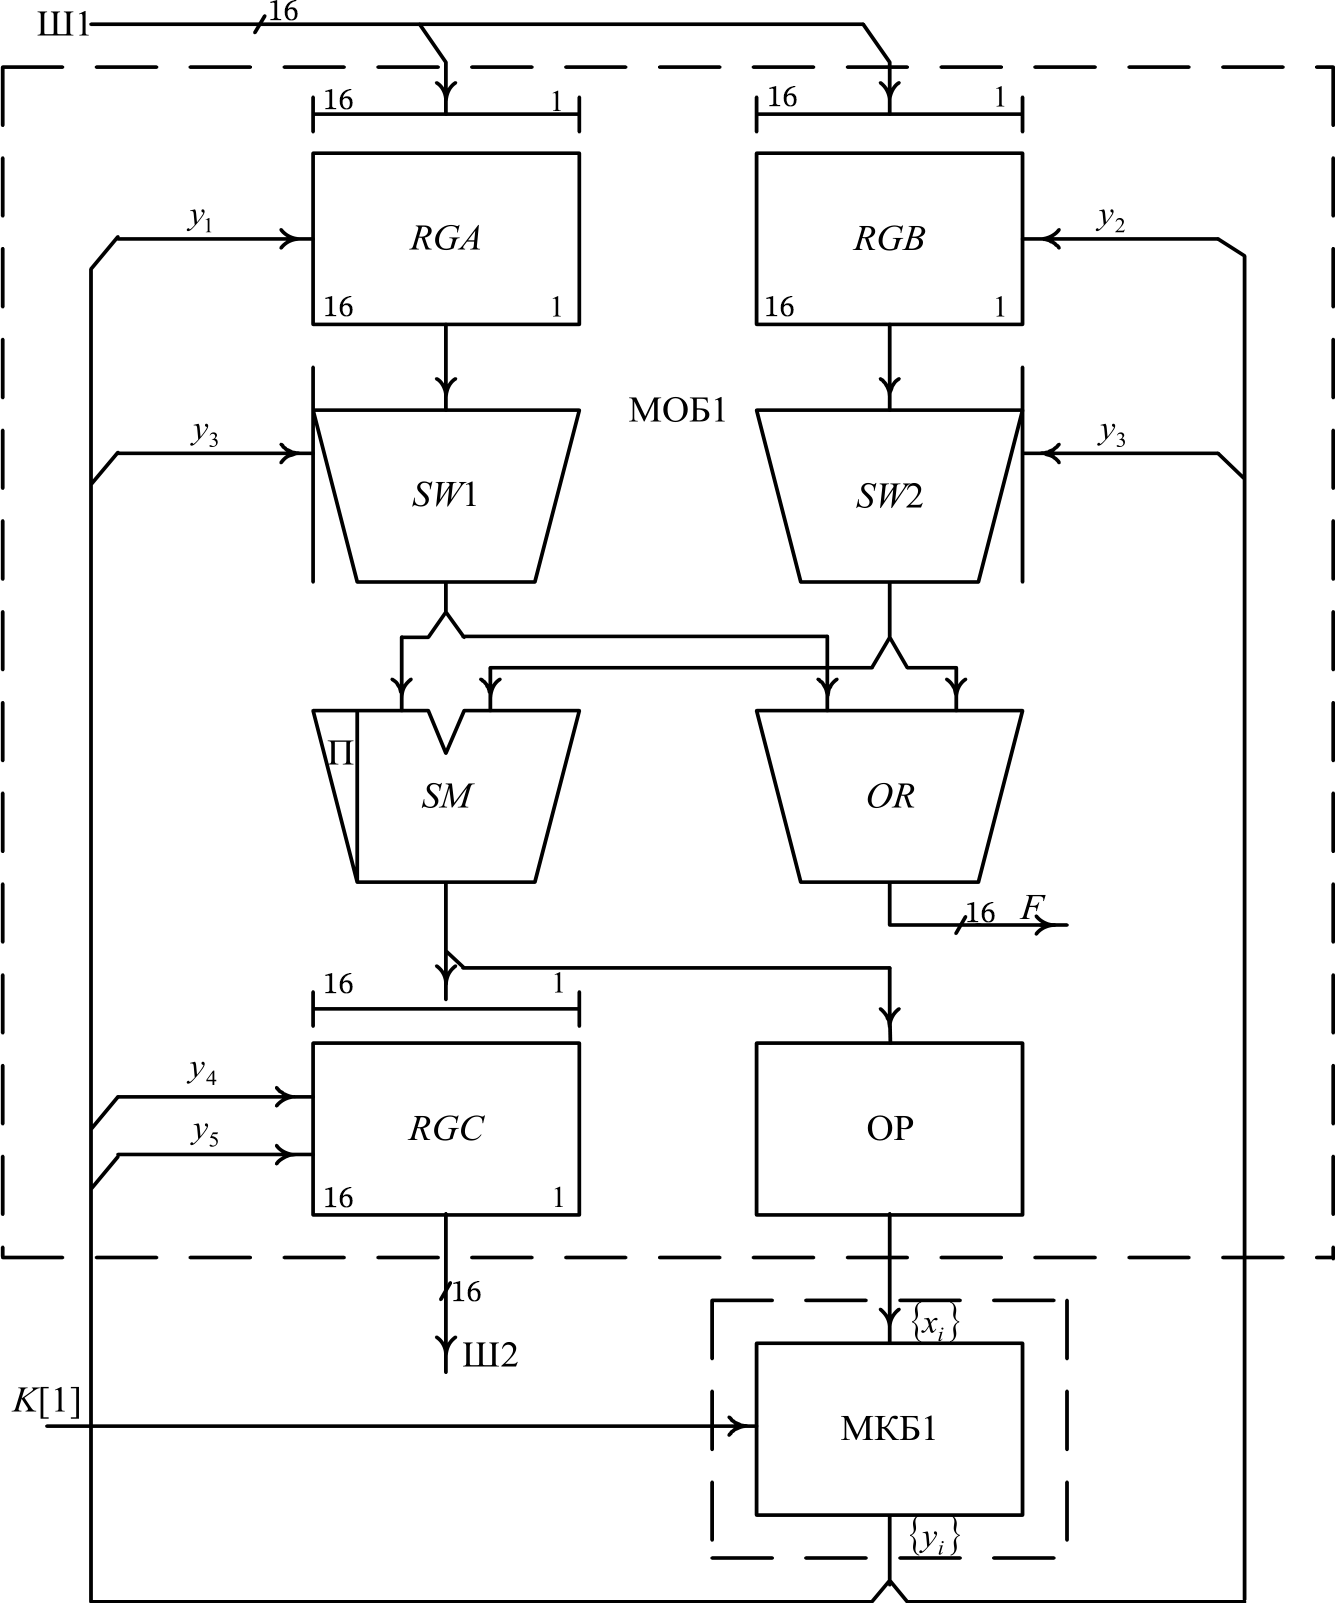
\includegraphics[height = 16\baselineskip]{./assets/01-operational-part-functional-schematic-16bit.png}
				\caption{Функціональна схема для додавання чисел}
				\label{fig:01-operational-part-functional-schematic}
			\end{figure}

			Після закінчення операції керуючий автомат аналізує ознаки результату і встановлює значення відповідних тригерів ознак. Ознаки результату обчислюються за допомогою булевих виразів:
			\begin{IEEEeqnarray*}{rCl}
				\varphi_1 &=& \mathit{П} \land \barneg{\schel{SM}}[n]~\text{— додатний результат (знаки~$00$),}\\
				\varphi_2 &=& \mathit{П} \land \schel{SM}[n]~\text{— від'ємний результат (знаки~$11$),}\\
				\varphi_3 &=& \barneg{\mathit{П}} \land \schel{SM} \lor \mathit{П} \land \barneg{\schel{SM}}[n]~\text{— переповнення розрядної сітки~(знаки~$01$ чи~$10$),}\\
				\varphi_4 &=& \bigwedge\limits_{i = 1}^{n + 1} \barneg{\schel{SM}}[i]~\text{— нульовий результат}.
			\end{IEEEeqnarray*}

			Ознака переповнення перевіряється до закінчення операції і за її наявності виконання програми переривається. Перевірка ознаки~\textit{OR} реалізується за допомогою 16~логічних 2-входових елементів~АБО за співвідношенням:
			\begin{IEEEeqnarray*}{rCl}
				F_i = A_i \lor B_i, \quad i = \{1, \dots, 16\},
			\end{IEEEeqnarray*}
			де $F_i$~— $i$-й вихід вузла логічного додавання. Ця операція виконується автоматично незалежно від коду команди.

		\subsection{Розробка мікропрограми додавання}
			За словесним алгоритмом додавання двійкових чисел у доповняльних кодах запишемо мікропрограму~(алг.~\ref{alg:01-addition}). Отримана мікропрограма дозволяє скласти змістовний граф мікропрограми~(рис.~\ref{fig:summation-algorithm-meaningful-graph}). В свою чергу отриманий змістовний граф мікропрограми кодується та розмічуюється. В результаті отримуємо закодований граф мікропрограми~(рис.~\ref{fig:summation-algorithm-encoded-graph}).
			\begin{algorithm}
				\caption{Додавання двійкових чисел}
				\label{alg:01-addition}
				\eIf(\tcc*[f]{$K[1]$~— однорозрядний код команди додавання}){$K[1]$}{
					$\schel{RGA} \coloneqq A$\tcc*{Приймання першого операнда}
					$\schel{RGB} \coloneqq B$\tcc*{Приймання другого операнда}
					$\schel{SM} \coloneqq A + B$\tcc*{Додавання}
					\eIf{$\varphi_3$}{
						$T_{\text{П}} \coloneqq \text{ПП}$\tcc*{Тригеру переповнення $T_{\text{П}}$ присвоюється ознака~ПП}
					}{
						$\schel{RGC} \coloneqq \schel{SM}$\tcc*{Присвоєння результату}
						$\schel{Ш2} \coloneqq \schel{RGC}$\tcc*{Пересилання в пам'ять}
					}
					}{
						Чекати\;
				}
			\end{algorithm}

			\begin{figure}[!htbp]
			\centering
				\includegraphics{assets/01-summation-algorithm-meaningful-graph.tikz}
			\caption{Змістовний граф мікропрограми додавання}
			\label{fig:summation-algorithm-meaningful-graph}
			\end{figure}

			\begin{figure}[!htbp]
			\centering
				\includegraphics{assets/02-summation-algorithm-encoded-graph.tikz}
			\caption{Закодований граф мікропрограми додавання}
			\label{fig:summation-algorithm-encoded-graph}
			\end{figure}

		\subsection{Розробка схеми модуля операційного блока}
			Отримані дані дозволили розробити модуль операційного блока~(рис.~\ref{fig:02-summation-principal-schematic}).
			\begin{figure}[!htbp]
				\centering
				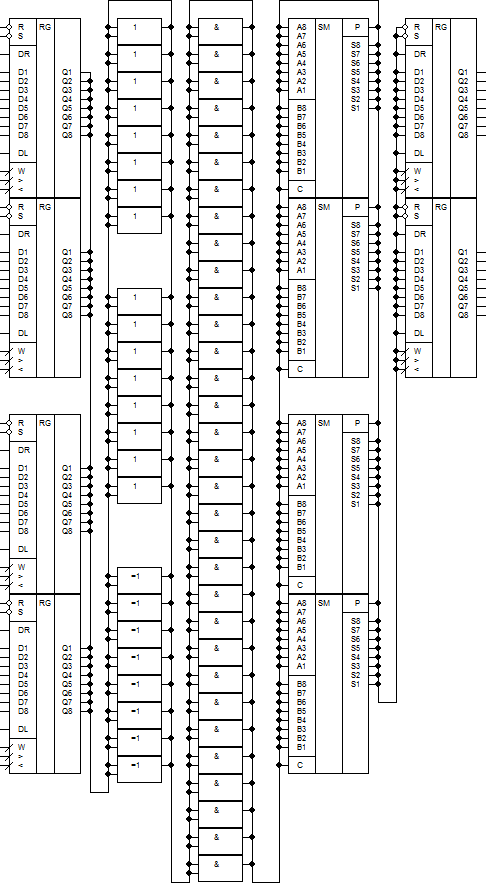
\includegraphics[height = 38\baselineskip]{./assets/02-summation-principal-schematic.png}
				\caption{Схема модуля операційного блока}
				\label{fig:02-summation-principal-schematic}
			\end{figure}

			Розроблений модуль операційного блока складається з таких елементів:
			\begin{enumerate}
				\item Регістри для зберігання операндів.
				\item Мікросхеми логічного АБО для реалізації порозрядної диз'юнкції над кодами операндів~$A$ і~$B$.
				\item Мікросхеми логічного І для підключення виходів регістрів до входів суматора.
				\item Мікросхеми логічного виключного АБО для створення старшого знакового розряду суматора і логічної ознаки~$\varphi_3 = x_1$ та~$\barneg{x_1}$.
				\item Вихідний регістр для приймання результату додавання та його передачі на вихідну шину.
				\item Суматори для виконання операції додавання.
			\end{enumerate}

		\subsection{Проектування керуючого блоку}
			% Закодований граф мікропрограми дозволяє побачити, що максимальна кількість станів автомата~$L = 8$. Для реалізації такої кількості станів необхідно і~достатньо використати $n = \ceil*{\log_2{8}} = 3$~$D$-тригери. Закодуємо стани автомата Мілі значеннями виходів $D$-тригерів за принципом кодування Грея та зобразимо це відповідним чином на рисунку.
			Із закодованого графа мікропрограми видно, що максимальна кількість станів автомата~$L = 8$, тому для реалізації необхідно $n = \ceil*{\log_2{8}} = 3$~$D$-тригери. Закодуємо стани автомата значеннями виходів $D$-тригерів за принципом кодування Грея:
			\begin{IEEEeqnarray*}{rClrClrClrCl}
				z_1 &=& \barneg{Q_1} \barneg{Q_2} \barneg{Q_3}, \quad &
				z_2 &=& \barneg{Q_1} \barneg{Q_2}         Q_3, \quad &
				z_3 &=& \barneg{Q_1}         Q_2          Q_3, &
				z_4 &=& \barneg{Q_1}         Q_2  \barneg{Q_1}, \quad \\
				z_5 &=&         Q_3          Q_2  \barneg{Q_1}, \quad &
				z_6 &=&         Q_3          Q_2          Q_1, &
				z_7 &=&         Q_3  \barneg{Q_2}         Q_1, \quad &
				z_8 &=&         Q_3  \barneg{Q_2} \barneg{Q_1}.
			\end{IEEEeqnarray*}
			% На основі отриманих даних складаємо граф автомата Мілі для мікропрограми додавання~(рис.~\ref{fig:mealy-machine}), який інтерпретує складену мікропрограму додавання двох двійкових чисел у доповняльних кодах.
			На основі отриманих даних складаємо граф автомата Мілі~(рис.~\ref{fig:mealy-machine}).
			\begin{figure}[!htbp]
			\centering
				\includegraphics{assets/03-sum-mealy-machine.tikz}
			\caption{Граф автомата Мілі для мікропрограми додавання}
			\label{fig:mealy-machine}
			\end{figure}

			Отриманий граф автомата Мілі для мікропрограми додавання двох двійкових чисел у доповняльних кодах дозволяє скласти структурну таблицю переходів автомату Мілі~(табл.~\ref{tab:structured-transfer-table}), яка знадобиться для подальших обчислень і є більш наочною.
			\begin{table}[!htbp]
				\centering
				\caption{Структурна таблиця переходів автомата Мілі}
				\label{tab:structured-transfer-table}
				\begin{tabular}{*{9}{c}}
					\toprule
						$z_i$ & $k(z_i)$ & $z_j$ & $k(z_j)$ & $\left\{ x_i \right\}$ & $\left\{ y_i \right\}$ & $D_1$ & $D_2$ & $D_3$\\
					\midrule
						$z_1$ & $000$ & $z_1$ & $000$ & $\barneg{\beta_1}$ & $—$   & $0$ & $0$ & $0$\\
						$z_1$ & $000$ & $z_2$ & $001$ & $1$                & $y_1$ & $0$ & $0$ & $1$\\
						$z_2$ & $001$ & $z_3$ & $011$ & $1$                & $y_2$ & $0$ & $1$ & $1$\\
						$z_3$ & $011$ & $z_4$ & $010$ & $1$                & $y_3$ & $0$ & $1$ & $0$\\
						$z_4$ & $010$ & $z_5$ & $110$ & $1$                & $y_4$ & $1$ & $1$ & $0$\\
						$z_5$ & $110$ & $z_6$ & $111$ & $1$                & $y_5$ & $1$ & $1$ & $1$\\
						$z_6$ & $111$ & $z_7$ & $101$ & $1$                & $y_6$ & $1$ & $0$ & $1$\\
						$z_7$ & $101$ & $z_1$ & $000$ & $x_1$              & $y_9$ & $0$ & $0$ & $0$\\
						$z_7$ & $101$ & $z_8$ & $100$ & $\barneg{x_1}$     & $y_7$ & $1$ & $0$ & $0$\\
						$z_8$ & $100$ & $z_1$ & $000$ & $1$                & $y_8$ & $0$ & $0$ & $0$\\
						\bottomrule
				\end{tabular}
			\end{table}

			На підставі даних структурної таблиці переходів автомату Мілі для мікропрограми додавання записуємо системи логічних рівнянь. Для функцій збудження входів~$D$-тригерів:
			\begin{IEEEeqnarray*}{rCl}
				D_1 = z_4 \lor z_5 \lor z_6 \lor z_7 \barneg{x_2}, \quad
				D_2 = z_2 \lor z_3 \lor z_4 \lor z_5, \quad
				D_3 = z_1 \lor z_2 \lor z_5 \lor z_6.
			\end{IEEEeqnarray*}
			Перетворимо отримані функції до заданого елементного базису «І—НЕ»:
			% Перетворимо отримані функції до заданого у завданні елементного базису NAND («І—НЕ», тут і далі позначається символом~$\lnand$):
			\begin{IEEEeqnarray*}{rCl}
				D_1 &=& z_4 \lor z_5 \lor z_6 \lor z_7 \barneg{x_2}
				    = \barneg{z_4} \lnand \barneg{z_5} \lnand \barneg{z_6} \lnand \left( z_7 \lnand x_2 \right),\\
				D_2 &=& z_2 \lor z_3 \lor z_4 \lor z_5
				    = \barneg{z_2} \lnand \barneg{z_3} \lnand \barneg{z_4} \lnand \barneg{z_5},\\
				D_3 &=& z_1 \lor z_2 \lor z_5 \lor z_6
				    = \barneg{z_1} \lnand \barneg{z_2} \lnand \barneg{z_5} \lnand \barneg{z_6}.
			\end{IEEEeqnarray*}
			Рівняння для вихідних сигналів:
			\begin{IEEEeqnarray*}{rClrClrCl}
				y_1 &=& z_1, \quad &
				y_2 &=& z_2, \quad &
				y_3 &=& z_3, \\
				y_4 &=& z_4, \quad &
				y_5 &=& z_5, \quad &
				y_6 &=& z_6, \\
				y_7 &=& z_7 \barneg{x_1}, \quad &
				y_8 &=& z_8, \quad &
				y_9 &=& z_7 x_1.
			\end{IEEEeqnarray*}
			В результаті розробили функціональну схему керуючого автомату~(рис.~\ref{fig:control-automata-schematic}).
			\begin{figure}[!htbp]
			\centering
				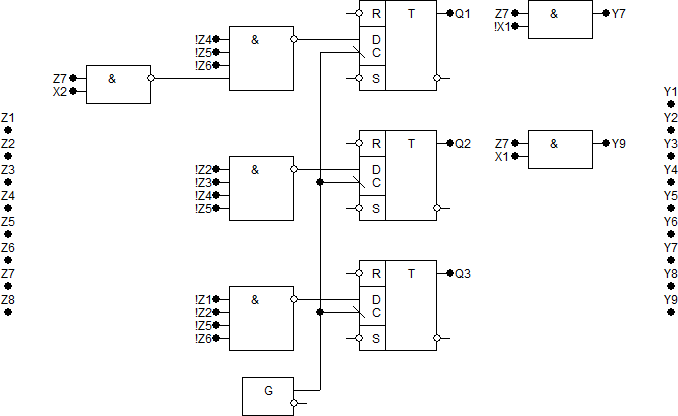
\includegraphics[width = \textwidth]{assets/control-schematic.png}
			\caption{Функціональна схема керуючого автомата}
			\label{fig:control-automata-schematic}
			\end{figure}

	\section{Висновок}
		Під час виконання даної розрахунково-графічної роботи ми навчились розробляти мікропрограми для виконання арифметично-логічних операцій, синтезувати за розробленим алгоритмом відповідні керуючі автомати та реалізовувати синтезовані автомати у вигляді функціональних схем.

\end{document}
